%%
%% This document created by A.Tasora
%%

\documentclass[final,3p]{elsarticle}


% to typeset URLs, URIs, and DOIs
\usepackage{url}
%\usepackage[T1]{fontenc}
\usepackage[utf8]{inputenc}
\usepackage[english]{babel}
\usepackage{hyperref}
\usepackage{amssymb}
\usepackage{amsmath}
\usepackage{amsthm}
\usepackage{cleveref}
\usepackage{bm}
\usepackage{mathtools}
\usepackage{siunitx}
\usepackage{subfig}
\usepackage{graphicx}
\usepackage{epstopdf}
\usepackage{tabularx}
\usepackage[ruled,vlined]{algorithm2e}  % ruled,vlined,linesnumbered
\usepackage{array}
\usepackage{booktabs}
\usepackage{multicol}
\usepackage{xcolor}
\usepackage[title]{appendix}
\usepackage{empheq}


\def\UrlFont{\rmfamily}

%% A.TASORA CUSTOM TEX COMMANDS:
%%
 
%\def\avect#1{{\boldsymbol{#1}}}
\def\amatr#1{{#1}}
\newcommand{\vect}[1]{\bm{#1}}
%\newcommand{\mat}[1]{#1}
\newcommand{\norm}[1]{\left\lVert#1\right\rVert}

\DeclareMathOperator*{\argmin}{arg\,min} % thin space, limits underneath in displays

\newtheorem*{definition*}{Definition}
\newtheorem{definition}{Definition}
\newtheorem*{remark*}{Remark}
\newtheorem{remark}{Remark}
\newtheorem*{theorem*}{Theorem}
\newtheorem{theorem}{Theorem}[section]
\newtheorem*{corollary*}{Corollary}
\newtheorem{corollary}{Corollary}[theorem]
\newtheorem{lemma}[theorem]{Lemma}


%%%%%%%%%%%%%%%%%%%%%%%%%%%%%%%%%%%%%%%%%%%%%%%%%%%%%%%%%%5


\begin{document}


%%
%% TITLE
%%


\title{Solving Cone Complementarity Problems in Non-Smooth Dynamics using the Alternating Direction Method of Multipliers}

%\author{Alessandro Tasora \\ alessandro.tasora@unipr.it}
\author{Alessandro Tasora}
\ead{alessandro.tasora@unipr.it}
\author{Simone Benatti}
\ead{simone.benatti@studenti.unipr.it}
\author{Dario Mangoni}
\ead{dario.mangoni@unipr.it}
\address{Universit\`a degli Studi di Parma, \\Dpt. of Engineering and Architecture\\Parco Area delle Scienze, 181/A, 43124 Parma, Italy }

% \affil[]{Universit\`a degli Studi di Parma, \\ 
% Dpt. of Engineering and Architecture, Parco Area delle Scienze, 181/A, 43124 Parma, Italy 
% \footnote{E-mail addresses: alessandro.tasora@unipr.it (A. Tasora), \\ simone.benatti@studenti.unipr.it (S. Benatti) dario.mangoni@studenti.unipr.it (D. Mangoni), rinaldo.garziera@unipr.it (R.Garziera).}
% }


\begin{abstract} 
This work discusses an efficient formulation of a geometrically exact three-dimensional beam which can be used in dynamical simulations involving large displacements, collisions and non-linear materials. To this end, we base our model on the shear-flexible Cosserat rod theory and we implement it in the context of Isogeometric Analysis (IGA). 
According to the IGA approach, the centerline of the beam is parameterized using splines; in our work the rotation of the section is parameterized by a spline interpolation of quaternions, and time integration of rotations is performed using the exponential map of quaternions. Aiming at an efficient and robust simulation of contacts, we propose the adoption of a non-smooth dynamics formulation based on differential-variational inequalities. 
The model has been implemented in an open-source physics simulation library that can simulate actuators, finite elements, rigid bodies, constraints, collisions and frictional contacts. 
This beam model has been tested on various benchmarks in order to assess its validity in non-linear static and dynamic analysis; in all cases the model behaved consistently with theoretical results and experimental data. 
\end{abstract}

\begin{keyword}
ADMM \sep non-smooth dynamics \sep contact
\end{keyword}


\maketitle              % typeset the title of the contribution

\begin{abstract}
We propose to use the Alternating Direction Method of Multipliers (ADMM) for solving the variational inequality that arises in non-smooth contact problems in multibody simulations. The ADMM method is based on simple computational primitives and offers good convergence properties especially for scenarios where loose tolerance on the precision can be accepted, thus making it attractive also for real-time applications. The method scales well with the problem size and require a small number of tuning parameters. Differently from other methods known in literature, such as fixed point iterations, it can easily handle problems that mix finite elements and rigid bodies, and it is only marginally affected by odd mass ratios or ill-posed problems. Another attractive feature is that it can be easily warm-started.
\end{abstract}
%
\begin{keyword}
ADMM \sep non-smooth dynamics \sep contact
\end{keyword}



%%%%%%%%%%%%%%%%%%%%%%%%%%%%%%%%%%%%%%%%%%%%%%%%%%%%%%%%%%%%


\section{Introduction}

Following the seminal works by Moreau 
\cite{mor88,Jean1992} 
most formulations for non-smooth dynamical problems are based on Measure Differential Inclusions (MDI): just like differential inclusions they allow set-valued force laws (such as the Coulomb-Amontons dry friction model) but also generalize to the case where velocity is assumed to be a possibly discontinuous function of bounded variation in order to allow impulsive events.

These problems can be solved by means of special time stepping methods that offer superior robustness and stability at the cost of solving a complementarity problem, or more in general a Variational Inequality (VI), per each time step
 \cite{acary2008numerical}. 
In this context, unknowns to be solved are velocity measures and reaction impulses at contact points and at joints: in cases of many parts with lot of frictional contacts, the large dimension of the VI could lead to a bottleneck in the time stepping process. This stimulated lot of research on efficient numerical methods in the last three decades.  

One of the former approaches, presented in 
\cite{StTr95}  % LCP solved via Lemke
, was based on solving a Linear Complementarity Problem (LCP) per each time step. LCPs are sub cases of VIs, for whom a direct method (Lemke algorithm) does exist. However, direct LCP solvers offer exact solution at the cost of very expensive pivoting sub iterations that scale badly with increasing number of unknowns, and for these reason they are not much used nowadays.

On the other hand, approximate but efficient methods based on fixed-point iterations became popular in the area of real-time simulators and robotics \cite{Bender2014}.
In most cases they are based on stationary methods like Gauss-Seidell or Jacobi iterations interleaved with projections on friction cones. They can be used to solve the LCP or the Cone Complementarity Problem (CCP), another special case of the VI in which the multibody contact problem can be formulated.
Attempts were made in order to parallelize them and to increase their convergence, such as over-relaxation, Krasnoselskii-Mann smoothing and warm starting, 
\cite{massSplittingRichard2012,TasoraAnitescuCMAME10} % P-GS iteration
but in general they perform poorly when there are odd mass ratios, and when articulated mechanisms such as robots are added to the scenarios - in those cases convergence often stalls, and if the iteration is prematurely truncated, reaction impulses are badly estimated and mechanisms fall apart or bend, and objects might interpenetrate. 

Another option is to solve the CCP as an optimization problem, using first-order optimization methods such as 
the Nesterov accelerated projected gradient descend  
\cite{hammadTOG2015}
or the Barzilai-Borwein spectral projected gradient
\cite{heynIJNME2013}. These methods are based on a simple projection operator,  matrix-by-vector multiplications and inner products. Their convergence is better than for fixed points iterations, however they share with them the following issue: that they often require the building of a Delassus operator, a matrix that is easy to compute in efficient (factored and sparse) format if diagonal masses are used because these can be easily inverted, but hard to handle if finite elements are added to the problem, because they introduce stiffness and damping matrices whose inverse would be needed as well.

A further class of solvers is represented by non-smooth newton methods, such as the one presented in 
\cite{Macklin2019} % Non-smooth Newton Method
, that assume a generic Nonlinear Complemetarity Problem (NCP), again a sub case of a VI, and represent the NCP complementarity constraints using non-smooth functions like the Fisher-Burmeister function. A generalized non-smooth Newton method can be used to find the zero of the functions, at the cost of solving a linear system per each iteration.

Under mild assumptions, the VI can be stated as a convex CCP, that can be also cast as an optimization problem, namely a Quadratic Program (QP) with convex constraints \cite{anitescuTasora2008}. For such a class of optimization problems, one can use Interior Point Methods (IPMs), a class of solvers that share some similarities with the above mentioned non-smooth Newton methods - for example the solution of a saddle-point linear system is required at each iteration. IPMs offer the best theoretical convergence. However, their implementation is quite intricate, and despite the encouraging theoretical properties, in practice they do not scale well for large problems. Also, there are no reliable ways to warm-start them
\cite{Mangoni2018}
.

The Alternating Direction Method of Multipliers (ADMM) has been proposed in the 1970s 
\cite{Glowinski75} % [ ADMM invention ]
\cite{Gabay1976} % [ ADMM invention ]
as a practical way to solve constrained optimization problems by iterating over the minimization of two (not necessarily differentiable) objectives.
ADMM introduces auxiliary variables and cast the original problem as the minimization of a separable objective subject to a linear constraint between the original variables and the auxiliary variables. With a proper choice of auxiliary variables, the minimization of the separable function is obtained iterating on two distinct minimization steps of lower complexity. The method iterates updating primal variables, auxiliary variables and dual variables similarly to a fixed point iteration: as such, they compares less favorably to IPMs if one is interested in convergence to high precision, however recent developments showed that in practical scenarios they offer superior speed, scalability and robustness, moreover their structure map well into parallel computing architectures
 \cite{Boyd2011}. % [ ADMM general theory and development ].
These positive properties triggered a recent revival of ADMM and similar operator-splitting methods even as alternatives to IPMs, especially in distributed convex optimization with large-scale problems where moderate precision is acceptable
\cite{Cannon2019}. % [COSMO  conic operator splitting method for large convex problems].

ADMM methods have been used in many fields, for instance computer graphics 
 \cite{Zhang2019}
, computational fluid dynamics
 \cite{Gregson2014} % [ ADMM and fluid simulation, inverse problems ]
, simulation of deformable structures 
 \cite{Overby2017} % [ ADMM projective dynamics hyperelastic models ]
and contact dynamics 
 \cite{Daviet2020} % [ ADMM thin objects frictional contact ]
, to name a few.


Recent developments addressed the possibility of accelerating the ADMM method.
In 
 \cite{Goldfarb2013} % [ ADMM with acceleration, both convex (non-strongly-convex require step skipping), one differentiable]
an acceleration scheme has been proposed for special cases of symmetric ADMMs, and assuming that one of the two objectives is differentiable.
%
In 
 \cite{Goldstein2014} % [ ADMM and AMA with Nesterov. Convergence ok if both problems are strongly convex (non-strongly-convex require restarting), one is quadratic ].
the Nesterov acceleration method has been proposed for problems where at least one of the two objectives is quadratic, and under the assumption that both objectives are strongly convex; if the latter assumption is not guaranteed, restarting strategies are needed. 
%
In 
 \cite{Kadkhodaie2015} %  [ A2DM2 accelerated ADMM, strongly convex ]
a similar acceleration method has been proposed, with $\mathcal{O}(\frac{1}{k^2})$ convergence rate, but without the assumption that one of the objectives must be quadratic.
%
Other types of improvements, based on the Anderson fixed point acceleration, have been put forward in 
 \cite{Zhang2019} % [ ADMM + Anderson acceleration, computergraphics ].
 \cite{Ouyang2020} % [ ADMM + Anderson acceleration, using Douglas-Rachford splitting, computergraphics ]
, showing high performance in computer graphics applications.

Recent developments also focused on the possibility of parallelizing the ADMM iterations on GPU and parallel architectures
\cite{Schubiger2020} % [ GPU implementation of ADMM | no need to compute residuals each iteration | krylov solver each iteration ].
.

In
\cite{Stellato2020} % [OSQP: an operator splitting solver for quadratic programs].
a specialized ADMM method for quadratic problems with conic constraints has been presented: on the top of this method we develop a solver that can exploit the nature of non-smooth dynamical problems. An attractive property of such ADMM is that it requires the solution of a linear system per each iteration, but unlike IPMs, such linear system most often remains unchanged during the iterations, so a factorization can be reused multiple times with a great benefit in terms of speed.

In our embodiment, unknowns are primal variables (velocity measures) and dual variables (impulses in contact points and joints), the convex cone constraints stem from the Coulomb friction law, and the system matrix includes terms from the mass matrices and from the tangent stiffness/damping matrices (hence it is sparse, but not necessarily diagonal).

This paper will present a model for the non-smooth dynamics, it will show how to cast it as a QP with convex conic constraint, it will present the ADMM method to solve it, it will discuss practical implementation details and then it will show benchmarks.



%%%%%%%%%%%%%%%%%%%%%%%%%%%%%%%%%%%%%%%%%%%%%%%%%%%%%%%

\section{Definitions}

In this section we list some basic definitions that we will use in the rest of the paper. 

\begin{definition}
A \textit{second order cone}, also Lorentz cone, is a self-dual self-scaled symmetric cone defined as
\begin{equation}
\label{eq:lorentzcone}
\mathcal{K} 
= \left \{ (x_0,\vect{x}_1) \in \mathbb{R} \times \mathbb{R}^{p-1}: \norm{\vect{x}_1}_2 \leq x_0  \right \} 
\; =   -\mathcal{K}^*.
\end{equation}
\end{definition}

\begin{definition}
The \textit{dual cone} $\mathcal{K}^*$ of a set $\mathcal{K}$ in a vector space equipped with an inner product, is always convex and is defined as
\begin{equation}
\label{eq:dualcone}
\mathcal{K}^* 
= \left \{ \vect{y} \in \mathbb{R}^n: \left\langle \vect{y}, \vect{x} \right\rangle \geq 0 \quad \forall \vect{x} \in \mathcal{K}  \right \}.
\end{equation}
\end{definition}

\begin{definition}
The \textit{polar cone} is defined as
\begin{equation}
\label{eq:polarcone}
\mathcal{K}^\circ 
= \left \{ \vect{y} \in \mathbb{R}^n: \left\langle \vect{y}, \vect{x} \right\rangle \leq 0 \quad \forall \vect{x} \in \mathcal{K}  \right \} 
\; =   -\mathcal{K}^*.
\end{equation}
\end{definition}

\begin{definition}
The \textit{normal cone} to a closed convex set $\mathcal{K}$ at the point $\vect{x}\in\mathcal{K}$ is
closed and convex and is defined as
\begin{align}
\label{eq:normalcone}
\mathcal{N}_{\mathcal{K}}(\vect{x}) 
&= \{ \vect{y} \in \mathbb{R}^n : \left\langle \vect{y}, \vect{x} - \vect{z} \right\rangle \geq 0, \forall \vect{z} \in \mathcal{K} \} 
\end{align}
\end{definition}

\begin{definition}
The \textit{indicator function} of a subset $\mathcal{A} \in \mathcal{E}$ is a scalar function $I: \mathcal{E} \mapsto \mathbb{R}$
defined as:
\begin{equation}
\label{eq:indicator}
{I}_{\mathcal{A}}(\vect{x}) = 
\left\{ 
\begin{array}[pos]{l}
0     \;  \text{if} \; \vect{x} \in \mathcal{A} \\
\infty   \; \text{if} \; \vect{x} \notin \mathcal{A}
\end{array}
\right.
\end{equation}
\end{definition}

\begin{remark*}
The indicator function of any closed set is lower semicontinuous.
\end{remark*}


\begin{definition}
The \textit{subdifferential} $\partial f(\vect{x}_0)$ at $\vect{x}_0$ of a convex, possibly non differentiable scalar function $f: \mathbb{R}^n \mapsto \mathbb{R}$, is the closed convex set of all subgradients $\vect{g}$ at $\vect{x}_0$:
\begin{equation}
\label{eq:subdifferential}
\partial f(\vect{x}_0) = \left\{ \vect{g} : 
  f(\vect{x}) -  f(\vect{x}_0) \geq \left\langle \vect{g}, (\vect{x} - \vect{x}_0) \right\rangle \; \forall \vect{x} \in \mathcal{E} \right\}.
\end{equation}
\end{definition}

\begin{remark*}
The indicator function of any closed set is lower semicontinuous.
\end{remark*}

\begin{remark*}
The subdifferential is a set valued function $\partial f(\vect{x}): \mathbb{R}^n \rightrightarrows \mathbb{R}^n$ in general, but as a special case, if $f(\vect{x})$ is differentiable, $\partial f(\vect{x}) = \left\{ \nabla f(\vect{x}) \right\}$.
\end{remark*}

\begin{remark*}
The subdifferential of an indicator function of a convex set is also its normal cone:
%
\begin{equation}
\label{eq:sub_ind}
\partial {I}_{\mathcal{K}}(\vect{x}) = \mathcal{N}_{\mathcal{K}}(\vect{x}).
\end{equation}
\end{remark*}

\begin{definition}
The \textit{projection} of $\vect{y}$ on a nonempty closed convex set $\mathcal{E}$ is a $\mathbb{R}^n \rightarrow \mathbb{R}^n$ mapping defined as:
%
\begin{align}
\label{eq:projector}
\Pi_{\mathcal{E}}(\vect{y}) = \mathrm{argmin}_{\vect{x} \in \mathcal{E}} \norm{ \vect{x} - \vect{y} }^2_2
\end{align}
%
If $f(\vect{y})$ is the indicator function $I_{\mathcal{E}}(\vect{y})$ to a nonempty closed convex set ${\mathcal{E}}$, defined as in \eqref{eq:indicator}, then $\mathrm{prox}_{f}(\vect{y})$ is the orthogonal projection onto that set:
%
\begin{align}
\label{eq:projectorindicator}
\mathrm{prox}_{I_{\mathcal{E}}}(\vect{y})  = \Pi_{\mathcal{E}}(\vect{y}) 
\end{align}
\label{def:projection}
\end{definition}


%%%%%%%%%%%%%%%%%%%%%%%%%%%%%%%%%%%%%%%%%%%%%%%%%%%%%%%


\section{The non-smooth multibody model}

Different time stepping schemes have been proposed for MDIs, here we refer to the one discussed \cite{TasoraAnitescuCMAME10} without lack of generality. After regularization and convexification and discretization, the MDIs leads to a major numerical bottleneck to be solved at each time step: a (mixed) CCP with unknowns $\vect{v}$ and $\vect{\gamma}_\epsilon$: 

\begin{subequations}
	\begin{empheq}[left=\empheqlbrace]{align}
    H \vect{v} - \vect{k} - D_\epsilon \vect{\gamma}_\epsilon &= 0   \label{eq:ChronoMCCP_a} \\
    D_{\epsilon}^T \vect{v}  + \vect{b}_\epsilon &= \vect{u}_\epsilon   \label{eq:ChronoMCCP_b} \\
    -\Upsilon^{\circ} \ni \vect{u}_\epsilon  \quad \bot &\quad  \vect{\gamma}_\epsilon \in \Upsilon  \label{eq:ChronoMCCP_c}
	\end{empheq}
	\label{eq:ChronoMCCP}
\end{subequations}

where 
\begin{itemize}
		\item unknown $\vect{v}$ is the speed at the end of the time step $h$
		\item unknown $\vect{\gamma}_\epsilon$ is the reaction in contacts and bilateral joints, a vector-signed measure with Lebesgue decomposition in atomic parts (impacts) and continuous parts (continuous reactions)
    \item $H$ is a positive definite matrix containing $M$, the block-diagonal matrix of the masses and inertia tensors of the bodies; if stiff
		loads are added too (ex. when finite elements come into play) it becomes a block-sparse matrix including the tangent stiffness and damping matrices,
		for instance $H=M-{h^2}\nabla_q\vect{f}-{h}\nabla_v\vect{f}$ in case of the first-order time stepper in \cite{TasoraAnitescuCMAME10}
    \item $D_\epsilon$ is a sparse matrix, the transpose jacobian of all constraints
    \item $\vect{k}$ is a vector containing terms proportional to applied forces $\vect{f}$
    \item $\vect{b}$ is a vector containing constraint stabilization terms, among other things
    \item $\Upsilon$ is the Cartesian product of all cones of admissible constraint forces, $\Upsilon = \bigtimes_i \Upsilon_i$
    \item if a frictional contact is added, $\Upsilon_i \subset \mathbb{R}^3$ is a second order Lorentz cone with aperture proportional to friction coefficient
    \item if a bilateral constraint is added, $\Upsilon_i = \mathbb{R}$ and $\Upsilon^\circ_i = \{0\}$
    \item if a unilateral constraint is added, $\Upsilon_i = \mathbb{R}^+$ and $\Upsilon^\circ_i = \mathbb{R}^-$
    \item $\Upsilon^{\circ}$ is the polar cone, opposite of the dual cone, i.e. $\Upsilon^{*} = -\Upsilon^\circ$.
\end{itemize}

For more details on the model we refer to 
\cite{negrutSerbanTasoraJCND2017}. % Posing Multibody Dynamics with Friction and Contact as a Differential Complementarity Problem

Introducing the Schur complement 
\begin{align}
N=D_{\epsilon}^T H^{-1} D_{\epsilon}
\label{eq:schur_n}
\end{align}
and the vector
\begin{align}
\vect{r}_\epsilon = D_{\epsilon}^T H^{-1} \vect{k} + \vect{b}_\epsilon
\label{eq:schur_r}
\end{align}
such that
\[
\vect{u}_\epsilon = N \vect{\gamma}_\epsilon + \vect{r}_\epsilon \, , 
\]
one can also write the problem as the following CCP:
\begin{align}
    -\Upsilon^{\circ} \ni  N \vect{\gamma}_\epsilon + \vect{r}_\epsilon 
    \quad \bot \quad  
    \vect{\gamma}_\epsilon \in \Upsilon
	\label{eq:ChronoCCP}
\end{align}

This CCP corresponds exactly to a first order optimality condition of a convex quadratic program:
\begin{subequations}
	\begin{empheq}[box=\fbox]{align}
	\text{min} \quad & \frac{1}{2} \vect{\gamma}_\epsilon^T N \vect{\gamma}_\epsilon + \vect{r}^T_\epsilon \vect{\gamma}_\epsilon \\
	\text{s.t.} \quad & \vect{\gamma}_\epsilon \in \Upsilon
	\end{empheq}
	\label{eq:ChronoCCP_min}
\end{subequations}
%
and in fact, the CCP \eqref{eq:ChronoCCP} can be written in the more conventional language of the KKT optimality conditions on \textit{dual variables} $\vect{y}$ multipliers, for $\vect{y}=-\vect{u}_\epsilon$, and \textit{primal variables} $\vect{\gamma}_\epsilon$:
\begin{subequations}
	\begin{align}
    N \vect{\gamma}_\epsilon + \vect{r}_\epsilon + I \vect{y} &= \vect{0} \\
    \vect{\gamma}_\epsilon &= \vect{z} \\
    \Upsilon \ni \vect{z}  \quad \bot &\quad \vect{y} \in \Upsilon^\circ  
	\end{align}
	\label{eq:ChronoCCP_kkt}
\end{subequations}
After the convex program \eqref{eq:ChronoCCP_min} is solved by ADMM, one can compute 
\begin{align}
\vect{v} = H^{-1}( \vect{k} + \bar{D}_\epsilon \vect{\gamma}_\epsilon)
\label{eq:v_post}
\end{align}
with an immediate step. 


The ADMM method in \cite{Stellato2020} can be used to solve problems in the form
\begin{subequations}
	\begin{align}
    P \vect{x} + \vect{q} + A^T \vect{y} &= \vect{0} \\
    A \vect{x} - \vect{b} &= \vect{z} \\
    \mathcal{C} \ni \vect{z}  \quad \bot &\quad \vect{y} \in \mathcal{N}_{C}(\vect{z})
	\end{align}
	\label{eq:OQSP_kkt}
\end{subequations}
and one can see that \eqref{eq:ChronoCCP_kkt} is a special case of \eqref{eq:OQSP_kkt} where $A=I$, $P=N$, $\mathcal{C}=\Upsilon$, $\vect{q}=\vect{r}$, $\vect{x}=\vect{\gamma}_\epsilon$, $\vect{b}=\vect{0}$, where some optimizations can take place because of the structure of our problem.

% TO ADD IN EXTENDED VERSION
%The ADMM method requires a fast way to perform a projection $\Pi_{\Upsilon}$ onto the friction cones $\Upsilon$ and a fast way to solve a linear problem with the matrix $A$. 

We remark that the ADMM method just makes the assumption of $\Upsilon$ being convex, so the problem can be generalized to $\vect{\gamma}_\epsilon \in \mathcal{C}$ where $\mathcal{C}$ is a generic convex set and at the same time we assume an associated 
 \footnote{Not all dissipative constitutive models are associated, for example in some computational plasticity models the plastic flow might deviate respect to the normal to the yeld surface, and the Coulomb contact model itself is not associated -in fact the contact velocity $\vect{u}$ can range into a wider cone than the polar of the friction cone, but our DVI model compensates fur such effect. We will assume associated models heretofore, and we do not deal with non-associated models to avoid additional complexity for the moment.} 
flow $\vect{u}_\epsilon \in - \mathcal{N}_{C}(\vect{\gamma}_\epsilon)$. For instance, $\mathcal{C}$ could be a capped friction cone to represent plasticization of contacts, or a cone translated downward to represent possible adhesion in contact up to a threshold, or the Von Mises yield region if $\vect{\gamma}_\epsilon$ represent stresses in finite elements undergoing plasticization. 

Also, in sake of highest generality, in presence of finite elements one might need to use tangent stiffness matrices $K$ and damping matrices $D$ to accommodate an implicit integration scheme for stiff elements, and this means that the Schur complement would be computed as $N=D_{\epsilon}^T H^{-1} D_{\epsilon}$. Here $H$ is a linear combination of $M$, $K$, $D$ (depending on the integration scheme) and in general is not diagonal anymore. 




\section{The ADMM solver}




For variables $(\vect{x},\vect{z}) \in \mathbb{R}^m \times \mathbb{R}^n$, the ADMM methods solve constrained optimization problems with separable structure
\begin{subequations}
	\begin{align}
    \text{min} \quad  & f(\vect{x}) + g(\vect{z}) \\
	  \text{s.t.} \quad &  A \vect{x} + B \vect{z} - \vect{b} = \vect{0}
	\end{align}
	\label{eq:admm}
\end{subequations}
where $f : \mathbb{R}^{n_x}\rightarrow\overline{\mathbb{R}}$ and  $g : \mathbb{R}^{n_z}\rightarrow\overline{\mathbb{R}}$ are proper convex lower-semicontinuous functions,
and $A \in \mathbb{R}^{n_x \times n_y}$, $B \in \mathbb{R}^{n_z \times n_y}$ are linear operators.

The optimality conditions require that primal feasibility
\begin{align}
A \vect{x}^\star + B \vect{z}^\star - \vect{b} = \vect{0} \label{eq:primalfeasibility1}
\end{align}
and dual feasibility
\begin{subequations}
	\begin{align}
     0 \in \partial	f(\vect{x}^\star) + A^T \vect{y}^\star \label{eq:dualfeasibility1}\\
	   0 \in \partial	g(\vect{z}^\star) + B^T \vect{y}^\star \label{eq:dualfeasibility2}
	\end{align}
	\label{eq:admm}
\end{subequations}
must hold at the solution $(\vect{x}^\star,\vect{z}^\star,\vect{y}^\star)$, saddle point of the Lagrangian with dual variables $\vect{y} \in \mathbb{R}^{n_y}$.

By introducing an augmented Lagrangian
\begin{align}
\mathcal{L}_{\rho}(\vect{x},\vect{z},\vect{y})= f(\vect{x}) + g(\vect{z}) + \vect{y}^T (A \vect{x} + B \vect{z} - \vect{b}) + \frac{\rho}{2} \norm{A \vect{x} + B \vect{z} - \vect{b}}_2^2
\end{align}
the ADMM method converges to the solution $(\vect{x}^\star,\vect{z}^\star,\vect{y}^\star)$ by iterating over two distinct minimization problems as in the following loop:
\begin{align}
 \vect{x}^{k+1} &\in \argmin_{\vect{x}} \mathcal{L}_{\rho}(\vect{x},\vect{z}^k,\vect{y}^k) \label{eq:lag1}\\
 \vect{z}^{k+1} &\in \argmin_{\vect{z}} \mathcal{L}_{\rho}(\vect{x}^{k+1},\vect{z},\vect{y}^k) \label{eq:lag2}\\
 \vect{y}^{k+1} &= \vect{y}^{k} + \rho ( A \vect{x}^{k+1} + B \vect{z}^{k+1} - \vect{b} )
 \label{eq:admm_iters}
\end{align}
The convergence of such method has rate $\mathcal{O}\left(\frac{1}{k}\right)$.
Although the convergence is fast in the first iterations, it tends to deteriorate later as in most fixed-point iterations; however in practical scenarios where loose tolerances can be accepted, even this basic formulation of ADMM proves to be efficient and robust.

The performance of ADMM depends on the efficiency of the updates in \eqref{eq:lag1} and \eqref{eq:lag2}. We will design the method such that the step \eqref{eq:lag2} will correspond to a very efficient projection onto a cone with separable structure, whereas the only bottleneck will be \eqref{eq:lag1}, corresponding to a quadratic optimization to be solved with a linear system.


In order to rewrite \eqref{eq:ChronoCCP_min} as a sum of two functions as in \eqref{eq:admm}, we introduce 
$\vect{\gamma}_\epsilon \in \mathbb{R}^{n_c}$ as primal variables, 
$\vect{z} \in \mathbb{R}^{n_c}$ as auxiliary variables, 
we add $\vect{\gamma}_\epsilon - \vect{z} = \vect{0}$ as the linear constraint, 
we reformulate the $\vect{\gamma}_\epsilon \in \Upsilon$ constraint by adding a non-smooth penalty function given by the indicator function 
$\mathcal{I}_\Upsilon (\vect{z})$,
and finally we have
\begin{subequations}
	\begin{align}
    \text{min} \quad & \frac{1}{2} \vect{\gamma}_\epsilon^T N \vect{\gamma}_\epsilon + \vect{r}^T_\epsilon \vect{\gamma}_\epsilon  
		+  \mathcal{I}_\Upsilon(\vect{z})  \\
	  \text{s.t.} \quad & \vect{\gamma}_\epsilon =  \vect{z}
	\end{align}
	\label{eq:admm_mod}
\end{subequations}

We can write the augmented Lagrangian introducing a step size parameter $\rho$ and a vector of dual variables $\vect{y}$, obtaining:
\begin{align}
\mathcal{L}_{\rho} \left(\vect{\gamma}_\epsilon,\vect{z},\vect{y} \right) &= 
\frac{1}{2} \vect{\gamma}_\epsilon^T N \vect{\gamma}_\epsilon + \vect{r}^T_\epsilon \vect{\gamma}_\epsilon  
+  \mathcal{I}_\Upsilon(\vect{z}) \nonumber \\
&+ \vect{y}^T (\vect{\gamma}_\epsilon - \vect{z}) 
+ \frac{\rho}{2} \norm{\vect{\gamma}_\epsilon - \vect{z}}_2^2
\end{align}
that is also, using the property $\vect{y}^T\vect{r} + \frac{\rho}{2}\norm{\vect{r}}_2^2 = \frac{\rho}{2}\norm{\vect{r}+\frac{1}{\rho} \vect{y}}_2^2 - \frac{1}{2\rho} \norm{\vect{y}}_2^2$, the following
\begin{align}
\mathcal{L}_{\rho} \left(\vect{\gamma}_\epsilon,\vect{z},\vect{y} \right) &= 
\frac{1}{2} \vect{\gamma}_\epsilon^T N \vect{\gamma}_\epsilon + \vect{r}^T_\epsilon \vect{\gamma}_\epsilon  
+  \mathcal{I}_\Upsilon(\vect{z}) \nonumber \\
&+ \frac{\rho}{2} \norm{\vect{\gamma}_\epsilon - \vect{z} + \frac{1}{\rho} \vect{y}}_2^2
- \frac{1}{2\rho} \norm{\vect{y}}_2^2
\label{eq:augmentedlagrangian}
\end{align}

The first step of ADMM requires to compute 
\begin{align}
\vect{\gamma}_\epsilon^{k+1} &= \argmin_{\vect{\gamma}_\epsilon} \mathcal{L}_{\rho} \left( \vect{\gamma}_\epsilon,\vect{z}^k,\vect{y}^k \right) \\
 &= \argmin_{\vect{\gamma}_\epsilon} \frac{1}{2} \vect{\gamma}_\epsilon^T N \vect{\gamma}_\epsilon + \vect{r}^T_\epsilon \vect{\gamma}_\epsilon  
+ \frac{\rho}{2} (\vect{\gamma}_\epsilon - \vect{z}^k + \frac{1}{\rho} \vect{y}^k)^T(\vect{\gamma}_\epsilon - \vect{z}^k + \frac{1}{\rho} \vect{y}^k)
- \frac{1}{2\rho} \norm{\vect{y}^k}_2^2 \\
 &= \argmin_{\vect{\gamma}_\epsilon} \frac{1}{2} \vect{\gamma}_\epsilon^T (N+ \rho I) \vect{\gamma}_\epsilon 
   + (\vect{r}_\epsilon - \rho \vect{z}^k + \vect{y}^k)^T \vect{\gamma}_\epsilon + C^k 
\end{align}

This is an unconstrained convex quadratic program whose KKT optimality conditions lead to the following linear problem:
\begin{align}
    \left[ N + \rho I \right] \vect{\gamma}_\epsilon^{k+1} =  \rho \vect{z}^k - \vect{r} - \vect{y}^k
		\label{eq:admm_1b}
\end{align}

%Optionally, following the idea of \cite{Stellato2020}, one could also introduce a small regularization parameter $\sigma$, that helps in case $N$ is near singular and $\rho$ is very small:
%\begin{align}
    %\left[ N + (\sigma+\rho) I \right] \tilde{\vect{\gamma}}_\epsilon = \sigma \vect{\gamma}_\epsilon^k + \rho \vect{z}^k - \vect{r} - \vect{y}^k
		%\label{eq:admm_1breg}
%\end{align}

The linear system \eqref{eq:admm_1b} can be solved as it is, but in our case it would be better to exploit the fact that the Schur matrix $N$ is a product $D_\epsilon^T H^{-1} D_\epsilon$. We would like to avoid computing $H^{-1}$, even storing a precomputed inverse for all iterations would be unpractical because often dense (except when $H$ is a diagonal mass matrix $M$). So we propose to replace \eqref{eq:admm_1b} with an equivalent saddle point problem: 

\begin{theorem}
\label{th:schurtokkt}
Let $\vect{\gamma}_\epsilon^{k+1}$ be a solution to \eqref{eq:admm_1b}, then it is also a solution to
%
\begin{subequations}
	\begin{align}
    \begin{bmatrix}
		 H   & D_\epsilon \\
		 D_\epsilon^T & - \rho I
		\end{bmatrix}
		\begin{Bmatrix}
		 \vect{v}^{k+1}   \\
		 -\vect{\gamma}_\epsilon^{k+1} 
		\end{Bmatrix}
		=
		\begin{Bmatrix}
		 \vect{k} \\
		 -\vect{b}_\epsilon + \rho \vect{z}^k -\vect{y}^k 
		\end{Bmatrix}
	\end{align}
	\label{eq:admm_1c}
\end{subequations}
%
\end{theorem}

\begin{proof}
Performing the multiplication of the upper part of the saddle point matrix one has 
$H \vect{v}^{k+1} - D_\epsilon \vect{\gamma}_\epsilon^{k+1} = \vect{k}$,
pre-multiplying by $H^{-1}$ one gets 
$\vect{v}^{k+1} = H^{-1} D_\epsilon \vect{\gamma}_\epsilon^{k+1} + H^{-1} \vect{k}$. 
The multiplication of the lower part gives 
$D_\epsilon^T \vect{v}^{k+1} + \rho I \vect{\gamma}_\epsilon^{k+1} = -\vect{b}_\epsilon + \rho \vect{z}^k -\vect{y}^k $, 
hence after substitution of $\vect{v}^{k+1}$ one gets
$D_\epsilon^T H^{-1} D_\epsilon \vect{\gamma}_\epsilon^{k+1}  + D_\epsilon^T H^{-1} \vect{k} + \rho I \vect{\gamma}_\epsilon^{k+1} = -\vect{b}_\epsilon + \rho \vect{z}^k -\vect{y}^k$. 
Recalling the definition of $N$ in \eqref{eq:schur_n} and the definition of $\vect{r}_\epsilon$ in \eqref{eq:schur_r}, this can be written also as 
$(N + \rho I) \vect{\gamma}_\epsilon^{k+1} =  \rho \vect{z}^k - \vect{r} - \vect{y}^k$. 
\end{proof}

\begin{corollary}
The linear system \eqref{eq:admm_1c} introduces an auxiliary variable $\vect{v} \in \mathbb{R}^{n_v}$, however the matrix is very sparse and does not require storing or computing any $H^{-1}$ matrix as we should do if using \eqref{eq:admm_1b}.
\end{corollary}

\begin{corollary}
A positive side effect of this approach is that its auxiliary variable $\vect{v}$ is also the velocity term in the original mixed CCP 
\eqref{eq:ChronoMCCP}, so one does not need to compute it as $\vect{v}=H^{-1}(\vect{k} + D_\epsilon \vect{\gamma}_\epsilon )$ after the iteration converged because it is already a byproduct of the linear solver in \eqref{eq:admm_1c}.
\end{corollary}

\begin{corollary}
If constraint compliance is added to the MDI, a compliance matrix $C_\epsilon$ can be present in the CCP, thus leading to a modified version of \eqref{eq:ChronoMCCP_b}:
\[
D_{\epsilon}^T \vect{v}  +C_\epsilon \vect{\gamma}_\epsilon + \vect{b}_\epsilon = \vect{u}_\epsilon
\]
In such case one would have $N=D_{\epsilon}^T H^{-1} D_{\epsilon} + C_\epsilon$, and \eqref{eq:admm_1c} would change into: 
\begin{subequations}
	\begin{align}
    \begin{bmatrix}
		 H   & D_\epsilon \\
		 D_\epsilon^T & - \rho I - C_\epsilon
		\end{bmatrix}
		\begin{Bmatrix}
		 \vect{v}^{k+1}   \\
		 -\vect{\gamma}_\epsilon^{k+1} 
		\end{Bmatrix}
		=
		\begin{Bmatrix}
		 \vect{k} \\
		 -\vect{b}_\epsilon + \rho \vect{z}^k -\vect{y}^k 
		\end{Bmatrix}
	\end{align}
	\label{eq:admm_1c_compl}
\end{subequations}
\end{corollary}



The second step of ADMM requires to compute 
\[
\vect{z}^{k+1} = \argmin_{\vect{z}} 
\mathcal{L}_{\rho} \left(\vect{\gamma}_\epsilon^{k+1},\vect{z},\vect{y}^k\right)
\] 
%
This is a minimization problem too, but it can be rephrased in terms of a projection on the $\Upsilon$ set, which has a separable structure.
In fact, recalling \eqref{eq:augmentedlagrangian} and removing constant terms: 
\begin{align}
\vect{z}^{k+1} &= \argmin_{\vect{z}}  
\mathcal{I}_\Upsilon(\vect{z}) 
+ \frac{\rho}{2} \norm{ \vect{\gamma}_\epsilon^{k+1} - \vect{z} + \frac{1}{\rho} \vect{y}^k}_2^2
\end{align}
%
Using the definition \ref{def:projection}, this leads to:
\begin{align}
\vect{z}^{k+1} &= \Pi_\Upsilon \left(  \vect{\gamma}_\epsilon^{k+1} +\frac{1}{\rho} \vect{y}^k \right )
\end{align}

Note that the projection $\Pi_\Upsilon$ can be performed efficiently in our case, because $\Upsilon$ is the Cartesian product of $n_c$ Coulomb second-order friction cones of lower dimension, assuming a set of $n_c$ contacts:
\[
\Upsilon = \Upsilon_1 \times \Upsilon_2 \times \ldots \times \Upsilon_{n_c}, \quad \Upsilon_i \subset \mathbb{R}^3
\]
The separable structure allows the projection to be performed as a tuple of simpler projections:
\[
\Pi_\Upsilon(\vect{p}) = \left\{ \Pi_{\Upsilon_1}(\vect{p}_1), \Pi_{\Upsilon_2}(\vect{p}_2), \ldots,  \Pi_{\Upsilon_{n_c}}(\vect{p}_{n_c}) \right\}, \quad \vect{p}_i \in \mathrm{R}^3
\]
%
Note that this requires an inexpensive and parallelizable operation.

A basic form of ADMM will then iterate over these updates:
\begin{align}
    \begin{bmatrix}
		 H   & D_\epsilon \\
		 D_\epsilon^T & - \rho I - C
		\end{bmatrix}
		\begin{Bmatrix}
		 \vect{v}^{k+1}   \\
		 -\vect{\gamma}_\epsilon^{k+1} 
		\end{Bmatrix}
		&=
		\begin{Bmatrix}
		 \vect{k} \\
		 -\vect{b}_\epsilon + \rho \vect{z}^k -\vect{y}^k 
		\end{Bmatrix} \label{eq:admm_step1} \\
		\vect{z}^{k+1} &= \Pi_\Upsilon \left(  \vect{\gamma}_\epsilon^{k+1} +\frac{1}{\rho} \vect{y}^k \right ) \label{eq:admm_step2} \\
		\vect{y}^{k+1} &= \vect{y}^k + \rho \left( \vect{\gamma}_\epsilon^{k+1} - \vect{z}^{k+1} \right) \label{eq:admm_step3}
\end{align}
%
Before being able to apply this iteration in real problems, we should introduce some optimizations that will make a big difference for the performance of the method, and that will be discussed in the next section.


\section{Implementation}


\subsection{Residuals and termination}

In order to monitor the convergence of the method, a measure of residual quantities must be introduced. 
Given the definitions \eqref{eq:primalfeasibility1},\eqref{eq:primalfeasibility1},\eqref{eq:primalfeasibility1}, one can define a primal and a dual residual as:
%
\begin{align}
 \vect{r}_{\text{primal}}^{k+1} &= \vect{\gamma}_\epsilon^{k+1}-\vect{z}^{k+1}   \\
 \vect{r}_{\text{dual}}^{k+1} &= N \vect{\gamma}_\epsilon^{k+1}+\vect{r}+\vect{y}^{k+1} 
\end{align}

An alternative way to compute $\vect{r}_{\text{dual}}^{k+1}$, that does not need to use the $N$ matrix, is 
\[
   \vect{r}_{\text{dual}}^{k+1} = D_\epsilon^T \vect{v}^{k+1} +C_\epsilon \vect{\gamma}_\epsilon^{k+1} + \vect{r} + \vect{y}^{k+1}
\]
Another option (see \cite{Boyd2011}) is to compute it as
\[
   \vect{r}_{\text{dual}}^{k+1} = \rho (\vect{z}^{k+1} - \vect{z}^{k})
\]
which is even faster, at the expense of storing the previous value of $\vect{z}$. 

The iteration is terminated when both $\vect{r}_{\text{primal}}$ and $\vect{r}_{\text{dual}}$ fall under prescribed tolerances. 

Here primal and dual residuals have an interesting physical interpretation: a large primal residual means that the solution provides reaction forces that do not satisfy the set inclusions (e.g. the friction might be overestimated), whereas a large dual residual means that the speed (in the contact point metric) is wrong. That is, in the discussed time stepping scheme, the measuring units of $\vect{r}_{\text{primal}}$ is the same of reaction impulses, e.g. \si{N.s}, whereas the measuring units of $\vect{r}_{\text{primal}}$ can be considered the same of speeds, e.g. \si{m/s}.

We remark that, depending on the measuring units, the two residual errors can have different importance: this means that it is useful to set two distinct tolerances $\epsilon_{\text{primal}}$ and $\epsilon_{\text{dual}}$. Different heuristics can be used to define relative tolerances too, as shown in \cite{Stellato2020}.


\subsection{Step size selection}

The basic method outlined in \eqref{eq:admm_step1}-\eqref{eq:admm_step3} uses a fixed step $\rho$. 

In general, small values of $\rho$ cause a fast reduction of the dual residual, but a slow reduction of the primal residual. This has a  physical interpretation: truncating iterations based on too small $\rho$ most often lead to solutions where parts do not interpenetrate, but some contact forces do not satisfy the inclusion in the Coulomb cone. That is, some parts might stick like contacts were glued.

On the other hand, large values of $\rho$ cause a fast reduction of the primal residual, but a slow reduction of the dual residual. This means that truncating iterations with too large $\rho$ most often lead to solutions where contact forces satisfy very well the inclusion in the Coulomb friction cones, but parts might interpenetrate.
 
Clearly, this calls for the introduction of a scheme that adaptively changes the step size $\rho$ in order to achieve a balanced reduction of both residuals.
In most cases one can use heuristics and adjust $\rho$ only one or two times during the iterations, hence allowing to reuse the factorization of the linear system \eqref{eq:admm_step1} as much as possible. In fact, the most time-consuming step is the factorization of the matrix in \eqref{eq:admm_step1}, but this happens only at the first iteration and at all iterations where $\rho$ changes, otherwise one can reuse the last factorization because the matrix is the same, and perform only the back solve step with the different right hand side. On average, in our tests, the back solve operation took less than $1/10$ of the time needed for the factorization. 

We tested different policies for scaling the $\rho$ step in our algorithm. 
All policies share the following concept: starting from an initial value $\rho_0$, the step is scaled once each $n_s$ iterations such that the primal and dual residuals are well balanced 
\cite{Wohlberg2017}, % [ a step size selection via residual balancing, scale residuals given problem measuring units]:
that is:
\begin{align}
	\rho^{k+1} = \rho^{k} \eta_\rho 
\end{align}
  
We define the \textit{balanced} scaling policy as
\begin{align}
	\eta_\rho = \frac{ \norm{\vect{r}_{\text{primal}}^{k}}_\infty }{ \norm{\vect{r}_{\text{dual}}^{k}}_\infty }  
\end{align}
We define the \textit{balanced normalized} scaling policy as
% this is the "balanced_fast" policy in our MATLAB code
\begin{align}
	\eta_\rho = \left( \frac{\norm{\vect{r}_{\text{primal}}^{k}}_\infty}{ \max{ \left( \norm{\vect{z}^k}_\infty,\norm{\vect{\gamma}_\epsilon^k}_\infty \right) } } \right)
															\left( \frac{\norm{\vect{r}_{\text{dual}}^{k}}_\infty}  { \norm{\vect{y}^k }_\infty }  \right)^{-1}
\end{align}

Another idea is presented in 
 \cite{Xu_adaptive_2017}, % [ Spectral stepsize selection as in Barzilai Borwein ]
where the the step is changed using the Barzilai-Borwein spectral formula. This is referenced as the \textit{spectral} scaling policy in the following.

In all the cases above, one needs safeguards to avoid excessive scaling, for example we limit the scaling factor $\eta_\rho$ by clamping it in the $\left[\frac{1}{50}, 50 \right]$ interval by default. Also, in order to avoid an excessive number of factorizations, one could force the scaling factor to $\eta_\rho=1$ (hence no change in $\rho$) if it is not too far from the unity anyway - for example by default we use a tolerance interval $\left[\frac{1}{2}, 2 \right]$, and if the scaling falls inside that interval, it is forced to $\eta_\rho=1$.


\subsection{Custom treatment of bilateral joints}

We experienced that it is possible to use a $\rho$ value that changes on a per-constraint basis. If one could know in advance which contact will be active at the solution, one could split $\rho_i$ values between very high or very low values for the fastest convergence, however this is not possible because the set of active constraints is known only at the solution. However, we still can use a
simple heuristics consisting in forcing a small value $\rho_b = 1e-9$ for bilateral constraints, where one knows in advance that the corresponding dual variable $y_i$ would be null anyway. This produces better convergence results in systems containing both contacts and many bilateral joints, such as when simulating articulated robots that grasp some objects. 

This means that, instead of using a scalar $\rho^{k}$, in our code we use a diagonal matrix $\Theta^{k}$ defined as:
\begin{align}
 \Theta_{i,j}^{k} = 
		\left\{
			\begin{matrix}
			0 & \mathrm{if} & i \neq j\\
			\rho_b & \mathrm{if} & i = j  \;  \mathrm{and} \; i \in \mathcal{C}_B \\
			\rho^{k} & \mathrm{if} & i = j  \;  \mathrm{and} \; i \notin \mathcal{C}_B \\
			\end{matrix}
		\right. 
\end{align}



		




\section{Final algorithm}

Using the above results, one can finally obtain the ADDM algorithm for solving the CCP of the non-smooth dynamics timestepper:

\begin{algorithm}
\DontPrintSemicolon
\KwIn{ Initial approximations $\vect{y}^0$, $\vect{z}^0$ }
\KwOut{ Solution $\vect{\gamma}_\epsilon^\star$, $\vect{v}^\star$, optionally also $\vect{y}^\star$, $\vect{z}^\star$ }
\SetKwFunction{StepAdjustPolicy}{StepAdjustPolicy}
\While{$i \leq n_{max iters}$}{
    $ \begin{bmatrix}
			 H   & D_\epsilon \\
			 D^T & - \Theta^k I - C_\epsilon
			\end{bmatrix}
			\begin{Bmatrix}
				\vect{v}^{k+1}  \\
			 -\vect{\gamma}_\epsilon^{k+1}
			\end{Bmatrix}
			=
			\begin{Bmatrix}
			 \vect{k} \\
			 -\vect{b}_\epsilon + \Theta^k \vect{z}^k - \vect{y}^k 
			\end{Bmatrix} $\;
	  $\vect{z}^{k+1} = \Pi_\Upsilon \left(  \vect{\gamma}_\epsilon^{k+1} +(\Theta^k)^{-1} \vect{y}^k \right )$ \;
		$\vect{y}^{k+1} = \vect{y}^k + \Theta^k \left( \vect{\gamma}_\epsilon^{k+1} - \vect{z}^{k+1} \right) $ \;
		$\vect{r}_{\text{primal}}^{k+1} = \vect{\gamma}_\epsilon^{k+1}-\vect{z}^{k+1}$ \;
		$\vect{r}_{\text{dual}}^{k+1}   = \Theta^k (\vect{z}^{k+1} - \vect{z}^{k})$ \;
		\If{$\norm{\vect{r}_{\text{primal}}^{k+1}} < \epsilon_{\text{primal}}$ and $\norm{\vect{r}_{\text{dual}}^{k+1}} < \epsilon_{\text{dual}}$ }{
			break \;
		}
		$\rho^{k+1} = $ \StepAdjustPolicy{$\rho^{k}$} \; 
		$\rho^{k+1} \rightarrow \Theta^{k+1}$ \;
}
%\Return{location}\;
\caption{The optimized ADMM algorithm}
\label{algo:admm1}
\end{algorithm}


The algorithm above contains a single computational bottleneck, that is the solution of the linear system. However, if a direct solver is used, a LU decomposition\footnote{In many cases the H matrix is hermitian, for example when just block-diagonal mass matrices are used, hence the decomposition of the symmetric indefinite saddle point matrix can be done via a LDL decomposition, which is faster than the LU decomposition. However there are cased where un-symmetric tangent stiffness matrices might be added to H, as happens in some finite element problems, precluding this optimization.} could be computed at the beginning and then recomputed only when the step size is adjusted, otherwise in all other iterations with $\rho^{k+1}=\rho^{k}$ the decomposition is unaltered and only a relatively inexpensive back solve is required.


\subsection{Preconditioning}

We experienced that the convergence of Algorithm \ref{algo:admm1} is negatively affected by the presence of odd mass ratios in the mechanical system. The immediate effect of uneven mass ratio is a broadening of the interval of singular values of the $N$ matrix. Note that this can be also a consequence of using different measuring units for different constraint multipliers $\gamma_i$, for instance even a system with odd mass ratios can have a badly conditioned $N$ matrix if some constraint reactions are assumed in newtons, other in kilo newtons - clearly, as the choice of measuring units is arbitrary, one should find a way to make the solver as much insensitive as possible to the scaling of the constraints. 

A possible remedy for this difficulty is to perform a simplified form of preconditioning by doing a diagonal scaling of $N$ and $\vect{r}_\epsilon$ before starting the iteration, thus operating on the scaled form of the problem:
%
\begin{align}
	\text{min} \quad & \frac{1}{2} \breve{\vect{\gamma}}_\epsilon^T \breve{N} \breve{\vect{\gamma}}_\epsilon + \breve{\vect{r}}^T_\epsilon \breve{\vect{\gamma}}_\epsilon \\
	\text{s.t.} \quad & \breve{\vect{\gamma}}_\epsilon \in \breve{\Upsilon} 
	\label{eq:ChronoCCP_min_scaled}
\end{align}
%
with $\breve{\vect{\gamma}}_\epsilon = S^{-1} \vect{\gamma}_\epsilon$, $\breve{N} = S N S$, 
$\breve{\vect{r}}^T_\epsilon = S \vect{r}^T_\epsilon$. 
We set $S_{ii} = \sqrt{\frac{1}{N_{ii}}}$. 
%As usual we avoid using directly $N$ and we rather compute
%\[
%N_{ii} = D_{\epsilon,i}^T H^{-1} D_{\epsilon,i} + C_{\epsilon,ii}
%\]
Note that other more advanced (and CPU intensive) preconditioners could be used, for example in \cite{Stellato2020} a modified Ruitz equilibration is proposed.  
After the solution is computed, one can quickly recover $\vect{\gamma}_\epsilon = S \breve{\vect{\gamma}}_\epsilon$. 

Note that in sake of high performance we never build explicitly $\breve{N}$ and $\breve{\vect{r}}^T_\epsilon$: what we need is just a scaling of the saddle point matrix involved in \eqref{eq:admm_step1}, that will simply include the scaled jacobians
$\breve{D}_\epsilon = S D_\epsilon$, the scaled compliance
$\breve{C}_\epsilon = S C_\epsilon S$,  the scaled term 
$\breve{\vect{b}}_\epsilon = S \breve{\vect{b}}_\epsilon$.

The preconditioned form of the ADMM algorithm, that we call P-ADMM heretofore, is not reported here for compactness: it is enough to replace the above scaled quantities in Agorithm \ref{algo:admm1}, where $\breve{\vect{\gamma}}_\epsilon,\breve{\vect{y}},\breve{\vect{z}}$ will replace $\vect{\gamma}_\epsilon, \vect{y}, \vect{z}$, then a final step is added after convergence, to recover the unscaled solution: $\vect{\gamma}_\epsilon = S \breve{\vect{\gamma}}_\epsilon$. Moreover, if one is interested in the residuals in the not-scaled original form, for instance to verify convergence, these can be computed as 
%
\begin{align}
\vect{r}_{\text{primal}}^{k+1} &= S \left( \breve{\vect{\gamma}}_\epsilon^{k+1}-\breve{\vect{z}}^{k+1} \right) \nonumber \\
\vect{r}_{\text{dual}}^{k+1}   &= S^{-1} \Theta^k (\breve{\vect{z}}^{k+1} - \breve{\vect{z}}^{k}) \nonumber
\end{align}


\subsection{Warm starting}

One of the nice properties of ADMM methods is that they can be easily warm started, something that for example is difficult to do with IPMs. 
This is a relevant feature in our context, because we must solve the problem \eqref{eq:ChronoCCP} at each time step, where one can expect some degree of temporal coherency in the values of $\vect{\gamma}_\epsilon$ between each step. This is especially true for simulations involving stacked objects, like when simulating environments for robots, granular flows or masonry buildings, because the contact forces often show limited changes over time, and the amount of contacts that change state can be limited. If so, one can reuse the last computed values of $\vect{\gamma}_\epsilon$ in the previous time step to warm-start the ADMM solver at the next time step.

This poses two difficulties. First of all, one must develop algorithms and data structures that are able to convey information from the contact at time $t_A$ to a time $t_B = t_A+h$. in fact, after ADMM computes the contact forces at step $t_A$, those could be saved into the contact data structures, however those contacts would be recomputed by the collision detection engine at the next time step $t_B$: since the objects move, also the contact manifold changes, thus it is not trivial to compute which contacts are persistent between the two steps. By using some heuristics and tolerances, one can detect if some contacts at time $t_B$ are the same contacts used at time $t_A$, if so, their last reaction forces $\vect{\gamma}_\epsilon$ can be copied to the new contacts and used for the warm starting, whereas completely new contacts are initialized with $\vect{\gamma}_\epsilon = 0$. 

Furthermore, one can see that the ADDM Algorithm \ref{algo:admm1} is a fixed point 
$\{\vect{y}^{k+1},\vect{z}^{k+1}\} = \vect{g} \left(\{\vect{y}^k,\vect{z}^k\}\right)$, thus one needs $\{\vect{y}^0,\vect{z}^0\}$ to warm start it, rather than $\vect{\gamma}_\epsilon^0$. This leads to two options: store both $\vect{y}$ and $\vect{z}$ values in the contact data (wasting some memory in case of large scale simulations, and complicating both data structures and bookkeeping) otherwise assume that the last ADMM run converged exactly up to $\vect{r}_{\text{primal}}=0$, so one could just store $\vect{\gamma}_\epsilon$ values in contacts, and then compute
%
\begin{align}
\vect{v}^0 &= H^{-1}( \vect{k} + D_\epsilon \vect{\gamma}_\epsilon^0) \nonumber \\
\vect{y}^0 &= - (D_\epsilon^T \vect{v}^0 + C \vect{\gamma}_\epsilon^0 + \vect{b}_\epsilon)  \nonumber \\
\vect{z}^0 &= \vect{\gamma}_\epsilon^0 \nonumber
\end{align}
This idea, implemented in Algorithm \ref{algo:admm2}, provides a speedup of 2x-10x in our tests.

\begin{algorithm}
\DontPrintSemicolon
\KwIn{ Initial approximation $\vect{\gamma}_\epsilon^0$, optional: $\vect{v}^0$}
\KwOut{ Solution $\vect{\gamma}_\epsilon^\star$, $\vect{v}^\star$, optionally also $\vect{y}^\star$, $\vect{z}^\star$ }
\SetKwFunction{ADMM}{ADMM}
\If{$\vect{v}^0$ is not provided}
{
	$\vect{v}^0 = H^{-1}( \vect{k} + D_\epsilon \vect{\gamma}_\epsilon^0)$ \;
}
$\vect{y}^0 = - (D_\epsilon^T \vect{v}^0 + C \vect{\gamma}_\epsilon^0 + \vect{b}_\epsilon)$ \;
$\vect{z}^0 = \vect{\gamma}_\epsilon^0$ \;
$\vect{\gamma}_\epsilon^\star, \vect{v}^\star = $ \ADMM{$\vect{y}^0$,$\vect{z}^0$} \; 
\caption{Warm-started ADMM}
\label{algo:admm2}
\end{algorithm}



% REMOVED - the overrelaxation form is not discussed
%** Using these results, and adding a Krasnoselskii-Mann relaxation factor $\alpha \in(0,2]$, one obtains the final algorithm:
%
%\begin{subequations}
	%\begin{align}
    %\begin{bmatrix}
		 %H   & D_\epsilon \\
		 %D^T & -(\sigma+\rho) I
		%\end{bmatrix}
		%\begin{Bmatrix}
		  %\tilde{\vect{v}}^{k+1}  \\
		 %-\tilde{\vect{\gamma}}_\epsilon^{k+1}
		%\end{Bmatrix}
		%&=
		%\begin{Bmatrix}
		 %\vect{k} \\
		 %-\vect{b}_\epsilon + \sigma \vect{\gamma}_\epsilon^k +\rho \vect{z}^k - \vect{y}^k 
		%\end{Bmatrix}
		%\\
		%\vect{\gamma}^{k+1}_\epsilon &=\tilde{\vect{\gamma}}_\epsilon^{k+1} + (1-\alpha) \vect{\gamma}_\epsilon^k \\
		%\vect{v}^{k+1} &=\tilde{\vect{v}}^{k+1} + (1-\alpha) \vect{v}^k \\
		%\vect{z}^{k+1} &= \Pi_\Upsilon \left( \alpha \tilde{\vect{\gamma}}_\epsilon^{k+1} + (1-\alpha) \vect{z}^k  + \frac{1}{\rho} \vect{y}^k \right) \\
		%\vect{y}^{k+1} &= \vect{y}^k + \rho \left( \alpha \tilde{\vect{\gamma}}_\epsilon^{k+1} + (1-\alpha) \vect{z}^k - \vect{z}^{k+1} \right) \\
		%\vect{r}_{\text{prim}} &= \vect{\gamma}_\epsilon^{k+1}-\vect{z}^{k+1} \\
		%\vect{r}_{\text{dual}} &= N \vect{\gamma}_\epsilon^{k+1}+\vect{r}+\vect{y}^{k+1} 
	%\end{align}
	%\label{eq:admm_final}
%\end{subequations}
%
%An interesting property of this formulation is that one does not need to recover $\vect{v} = \amatr{H}^{-1}(\vect{k}+\amatr{D}^T \vect)\vect{\gamma}^{k+1}$ at the end because, for $\alpha=1$, this is also a byproduct of the linear system solve as $\vect{v}= \tilde{\vect{v}}^{k+1}$.
%In case of $\alpha\neq1$, one needs to keep it updated as 
%$\vect{v}^{k+1} =\tilde{\vect{v}}^{k+1} + (1-\alpha) \vect{v}^k$; 
%but this also means that an initial value of $\vect{v}^0$, consistent with the initial value $\vect{\gamma}^0$, must be computed, hence before the iteration one has to initialize 
%\[
%\vect{v}^0 = \amatr{H}^{-1}(\vect{k} + \amatr{D} \vect{\gamma}^0)
%\]





\section{Benchmarks}



\subsection{High stack with odd mass ratio}

This benchmark represents a typical worst case scenario in non-smooth dynamics, where
a heavy object sits on a high stack of rigid bodies of much lower mass, as shown in Fig.\ref{fig:t6_snapshot}. The stable stacking
is already a demanding case for contact dynamics, but the presence of extremely odd mass ratios add a
further complication. 

To this end we designed two sub-cases: \textsc{Test 1.a} and \textsc{Test 1.b}. Both feature
a vertical stack of 20 spheres with mass $m=\SI{10}{kg}$ each, except the 10th sphere that has
a mass of $m=\SI{10000}{kg}$. A further sphere with mass $m=\SI{1000}{kg}$ is placed on the floor.
All rigid bodies are subject to a vertical gravitational field $g=\SI{9.8}{m/s^2}$. For \textsc{Test 1.a}
one has the analytical solution (all contacts are active). The \textsc{Test 1.b}
differs from \textsc{Test 1.a} in that the heavy sphere is pulled upward by a force twice its weight, hence
causing a separation at the contact below it.

As expected, in both \textsc{Test 1.a} and \textsc{Test 1.b} the projected Jacobi iteration, one of the most common
methods in non-smooth dynamics, has a very bad convergence rate \footnote{It is a known fact that the simulation 
of high stacks of objects is a major difficulty in non-smooth dynamics, especially in real-time simulators
and in video games where the projected fixed-point iterations are truncated to keep the computational
time within a limited frame budget. In those cases, the limited precision of the solution will lead to underestimated
contact forces, undesired slow interpenetration of the parts and, ultimately, to unnatural collapses of stacks.}.
As shown in Fig.\ref{fig:t6_convergence_b}, 
the ADMM method presented in this paper behave
much better than the projected Jacobi iteration and, interesting enough, it also converges faster
than the Preconditioned Spectral Projected Gradient with Fall-Back (P-SPG-FB), an
efficient method for non-smooth problems presented in \cite{hammadTOG2015}.

\begin{figure}[!tbp]
  \centering
  \begin{minipage}[t]{0.48\textwidth}
    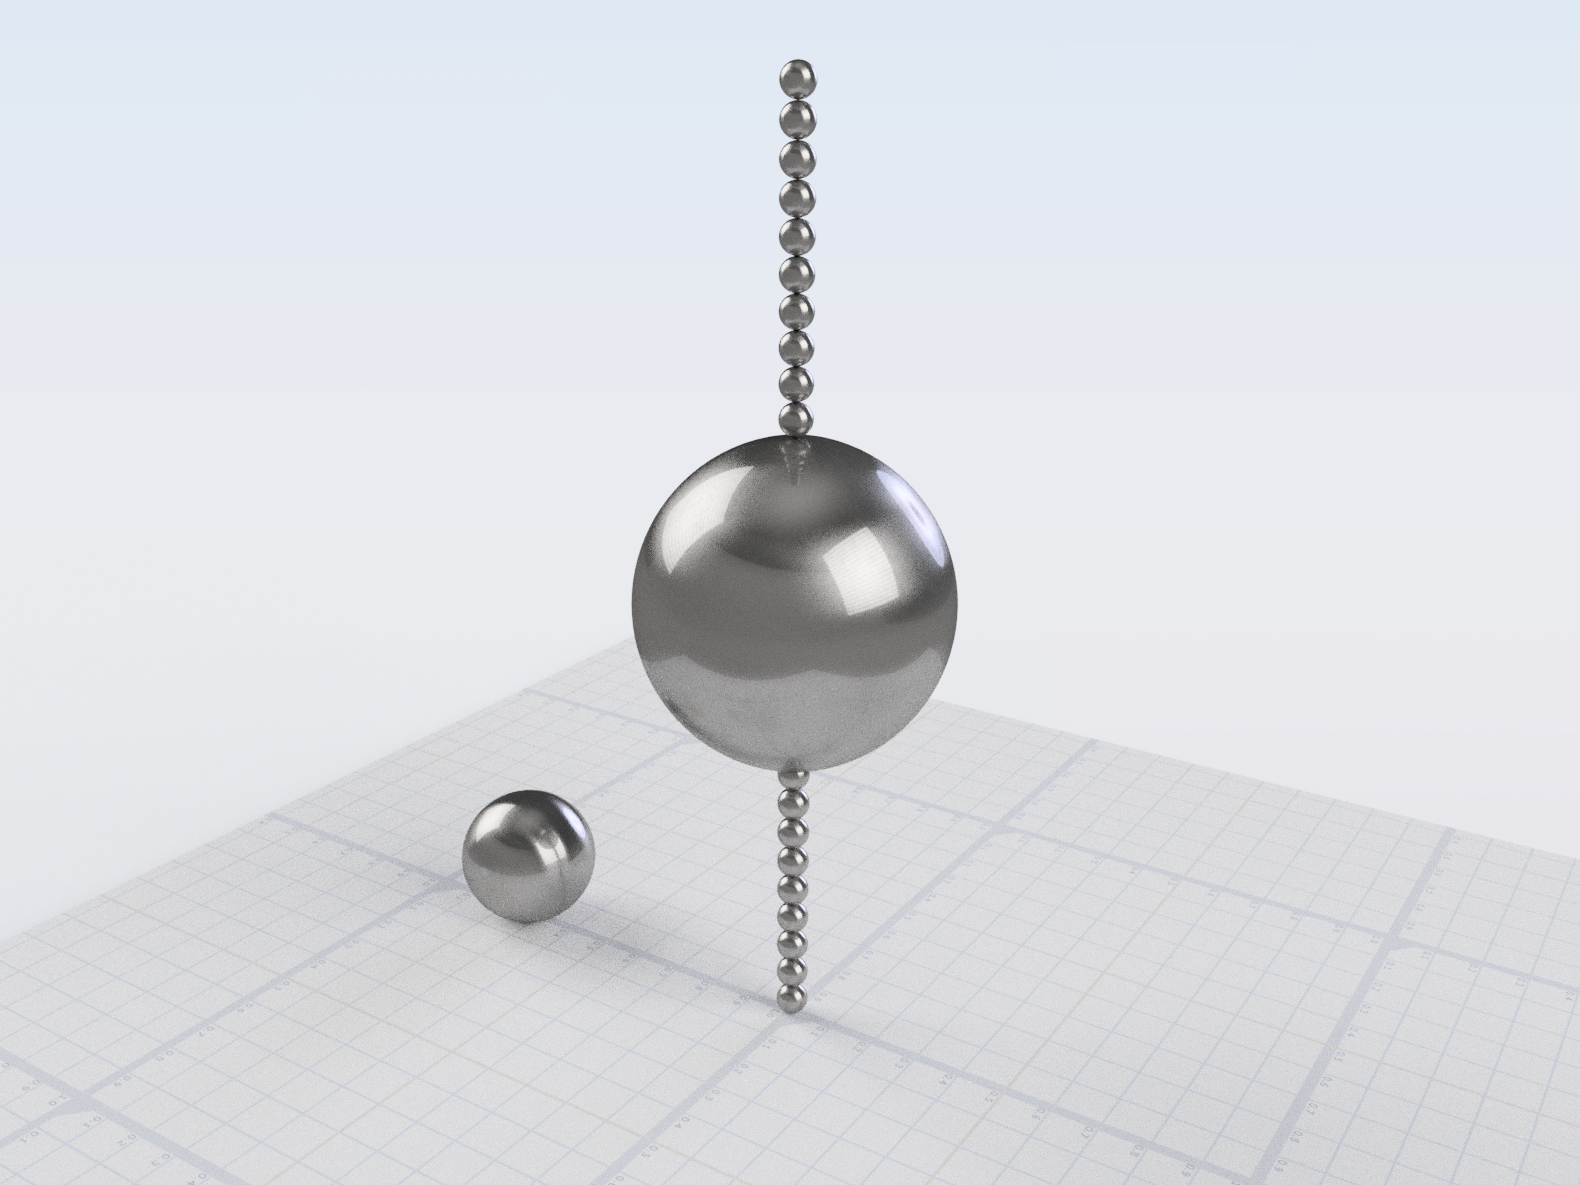
\includegraphics[width=\textwidth]{t6_snapshot.png}
    \caption{Setup of \textsc{Test 1}.}
		\label{fig:t6_snapshot}
  \end{minipage}
  \hfill
  \begin{minipage}[t]{0.48\textwidth}
    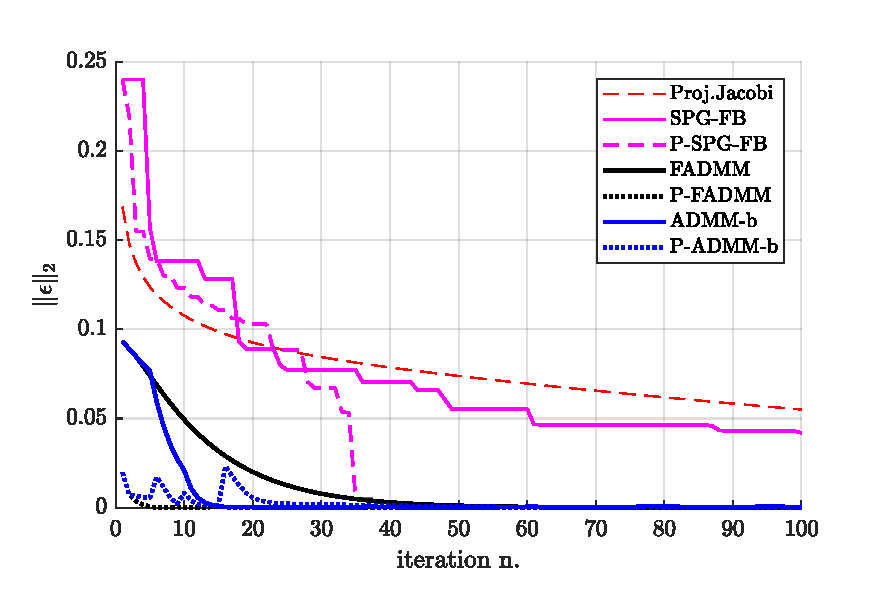
\includegraphics[width=\textwidth]{t6_convergence_b.pdf}
    \caption{Convergence of ADMM methods compared to the Jacobi projected fixed point iteration, for \textsc{Test 1.b} 
		The plot shows the violation of unilateral constraints in terms of penetrating residual velocity. }
		\label{fig:t6_convergence_b}
  \end{minipage}
\end{figure}

\begin{figure}[!tbp]
  \centering
  \begin{minipage}[t]{0.48\textwidth}
    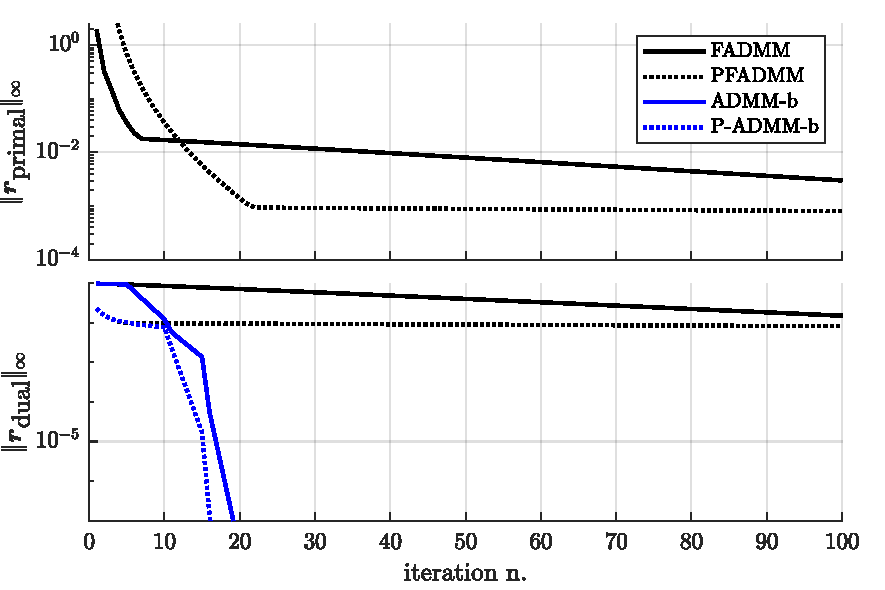
\includegraphics[width=\textwidth]{t6_primdual_a.pdf}
    \caption{Convergence of primal and dual residuals in \textsc{Test 1.a}.}
		\label{fig:t6_primdual_a}
  \end{minipage}
  \hfill
  \begin{minipage}[t]{0.48\textwidth}
    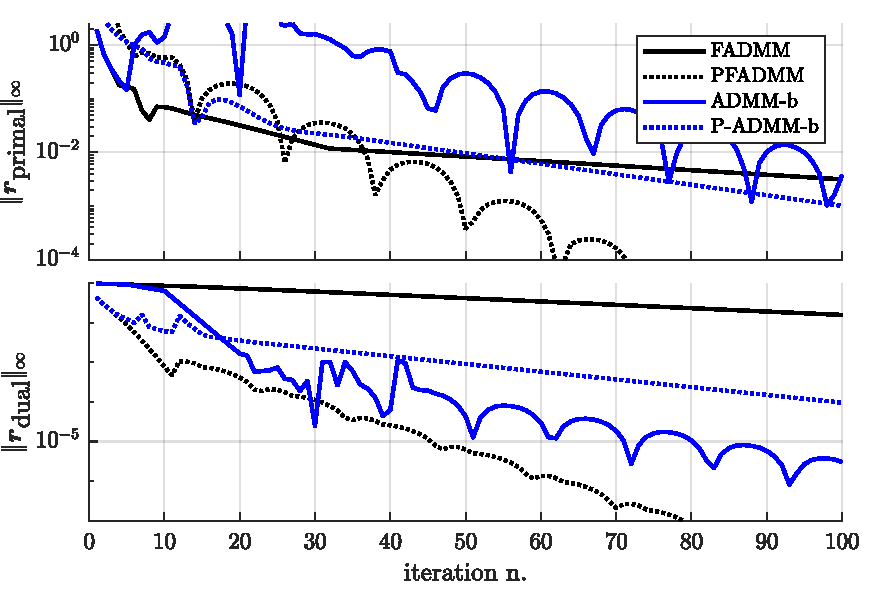
\includegraphics[width=\textwidth]{t6_primdual_b.pdf}
    \caption{Convergence of primal and dual residuals in \textsc{Test 1.b}. }
		\label{fig:t6_primdual_b}
  \end{minipage}
\end{figure}

For \textsc{Test 1.a}, Fig.\ref{fig:t6_primdual_a} shows that the ADMM method using the \textit{balanced} adaptive step size can converge to the exact solution in less than 20 iterations (the primal residual is not visible in the semilogarithmic plot as it is immediately zero from the first iteration). 

Note also that we force the update of the step every $n_s$ steps because each update of $\rho$ corresponds of a costly factorization of a large matrix.
Fig.\ref{fig:t6_primdual_a_ns} shows that, in this benchmark, the convergence improves for denser updates, 
meeting the tolerance in the same amount of updates: this would suggest using a small $n_s$ anyway. However, for more complex and randomized scenarios, 
we found that a good tradeoff is $n_s=5$. This tradeoff value can change depending on the speed of solver used for the factorization: the higher the performance
for the back solve respect to the factorization, the higher is the optimal $n_s$.

The FADMM method with the default fixed step $\rho=0.05$, instead, converges slowly. 
Repeating the FADMM test with different step sizes as shown in Fig.\ref{fig:t6_primdual_a_rho}, 
however, the convergence is greatly improved, suggesting that the FADMM method is sensitive to the initial choice of the time step. 

\begin{figure}[!tbp]
  \centering
  \begin{minipage}[t]{0.48\textwidth}
    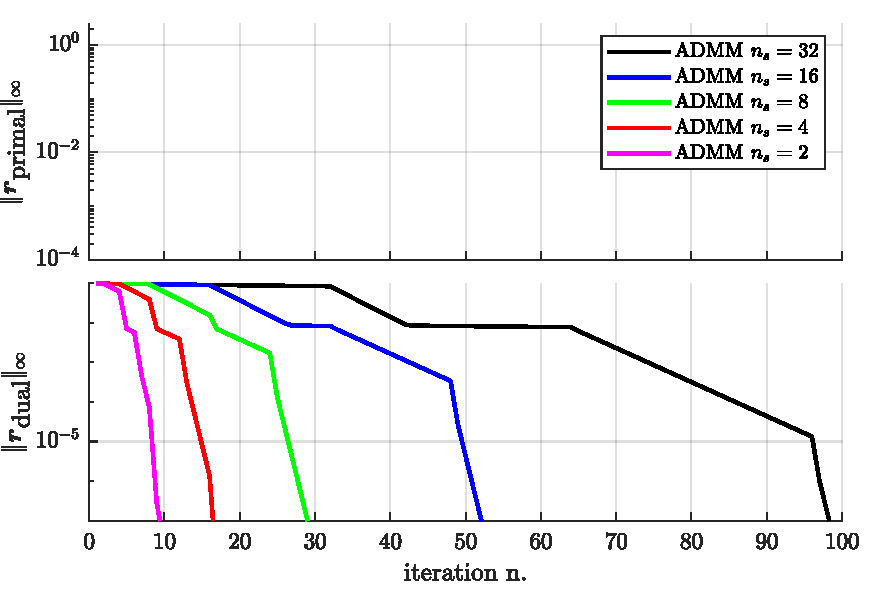
\includegraphics[width=\textwidth]{t6_primdual_a_ns.pdf}
    \caption{Convergence of primal and dual residuals in \textsc{Test 1.a} for varying frequency $n_s$ of automatic updates to the step size, in the ADMM algorithm.}
		\label{fig:t6_primdual_a_ns}
  \end{minipage}
  \hfill
	\begin{minipage}[t]{0.48\textwidth}
    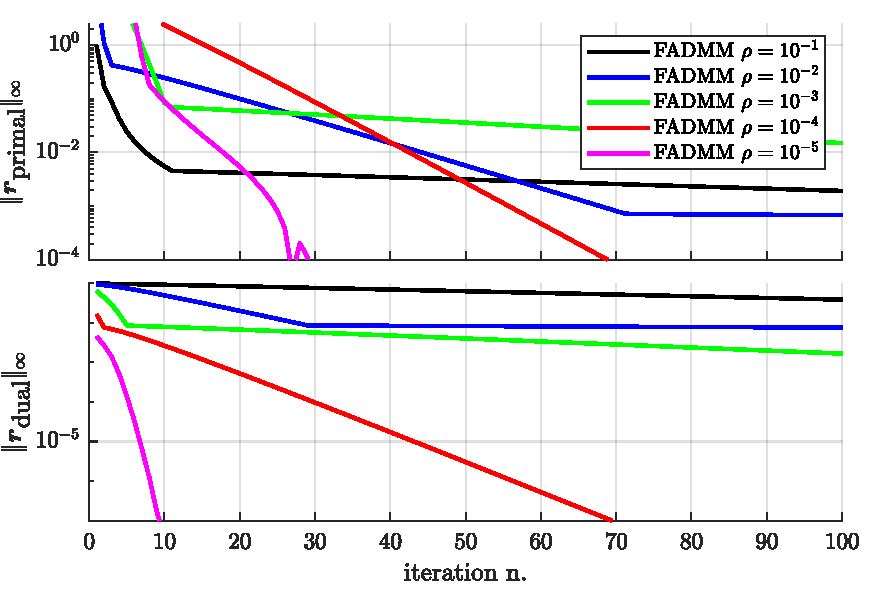
\includegraphics[width=\textwidth]{t6_primdual_a_rho.pdf}
    \caption{Convergence of primal and dual residuals in \textsc{Test 1.a} for varying values of the step size $\rho$ in the FADMM algorithm.}
		\label{fig:t6_primdual_a_rho}
  \end{minipage}
\end{figure}



For \textsc{Test 1.b}, convergence plots in Fig.\ref{fig:t6_primdual_b} show that the FADMM is very efficient even if starting from 
a fixed not optimal step size, although the performance deteriorates if no preconditioning is used. The ADMM method with balanced 
step adaptivity $n_s=5$ converges quite well, especially with the help of a preconditioner.

Showing that a solver is capable of handling this class of object-stacking problems is relevant, for instance,
to the field of civil engineering, because it shares the same difficulties of simulating tall masonry structures 
when assessing stability and seismic response via discrete elements \cite{Beatini2017}. 



\subsection{Bulldozer on stone slabs}

TO DO 



\begin{figure}[!tbp]
  \centering
  \begin{minipage}[t]{0.48\textwidth}
    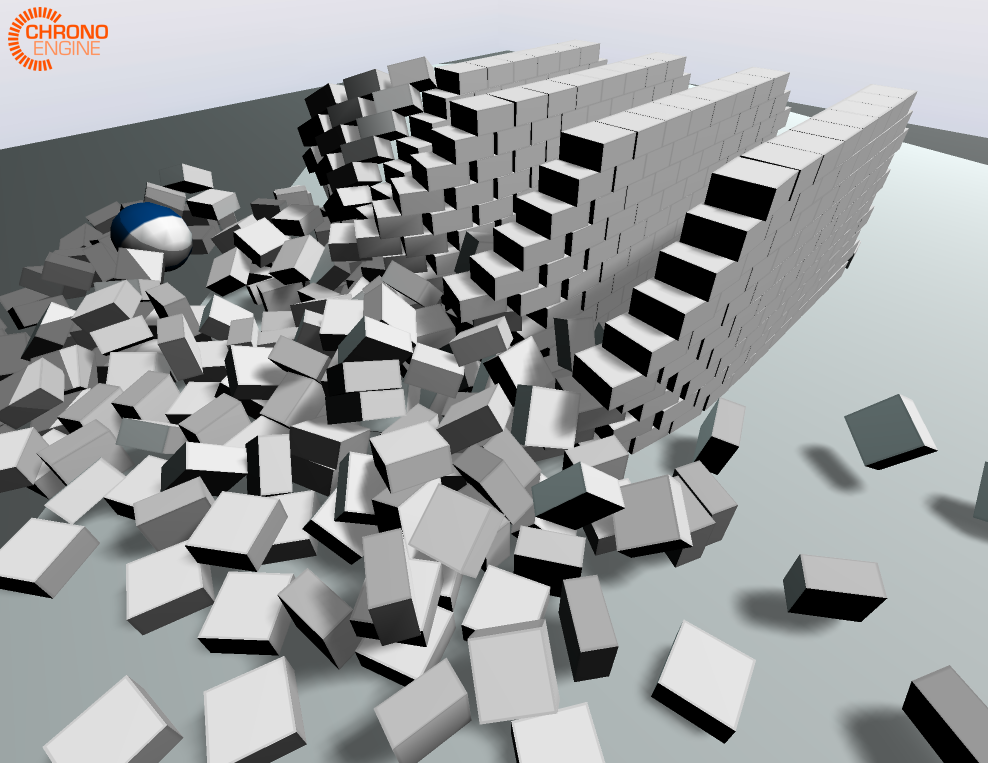
\includegraphics[width=0.8\textwidth, trim=0cm -3cm 0 3cm]{t8_snapshot.png}
    \caption{Snapshot from \textsc{Test 2}, the wrecking ball benchmark (600 bricks in four walls).}
		\label{fig:t6_primdual_a_ns}
  \end{minipage}
  \hfill
	\begin{minipage}[t]{0.48\textwidth}
    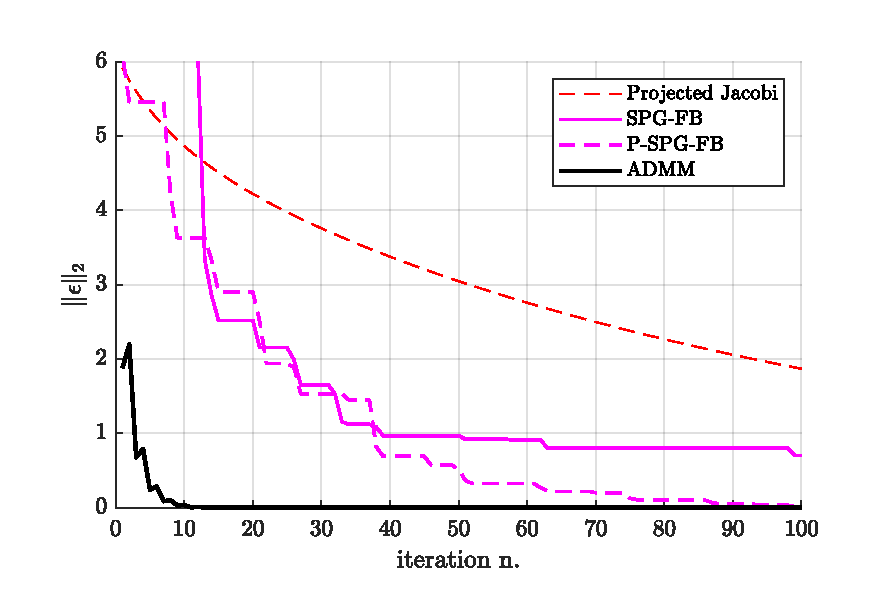
\includegraphics[width=\textwidth]{t8_convergence.pdf}
    \caption{Constraint violation compared to fixed point Jacobi iterations and to SPG methods, in \textsc{Test 2}.}
		\label{fig:t8_convergence}
  \end{minipage}
\end{figure}

\begin{figure}[!tbp]
  \centering
  \begin{minipage}[t]{0.48\textwidth}
    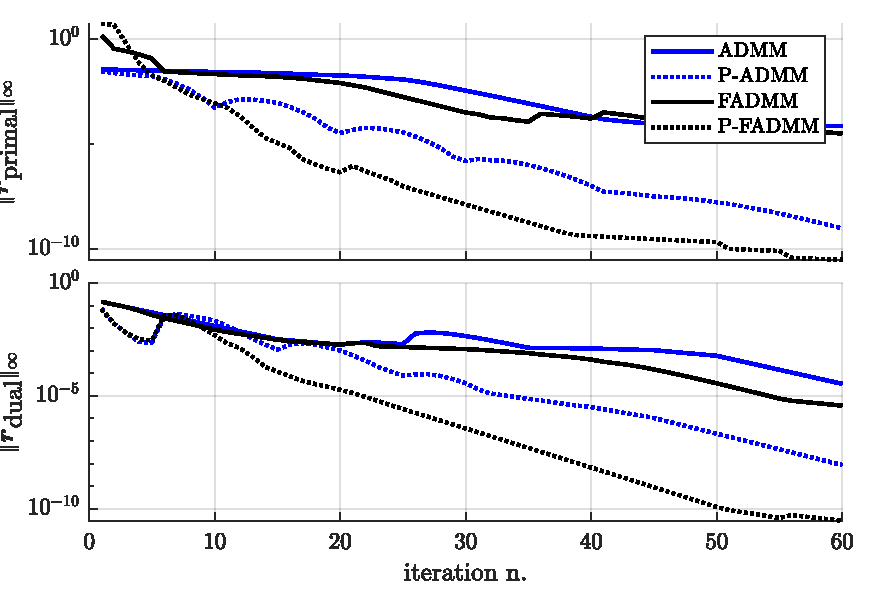
\includegraphics[width=\textwidth]{t8_primdual.pdf}
    \caption{Primal-dual convergence of the algorithm in \textsc{Test 2}.}
		\label{fig:t8_primdual}
  \end{minipage}
  \hfill
	\begin{minipage}[t]{0.48\textwidth}
    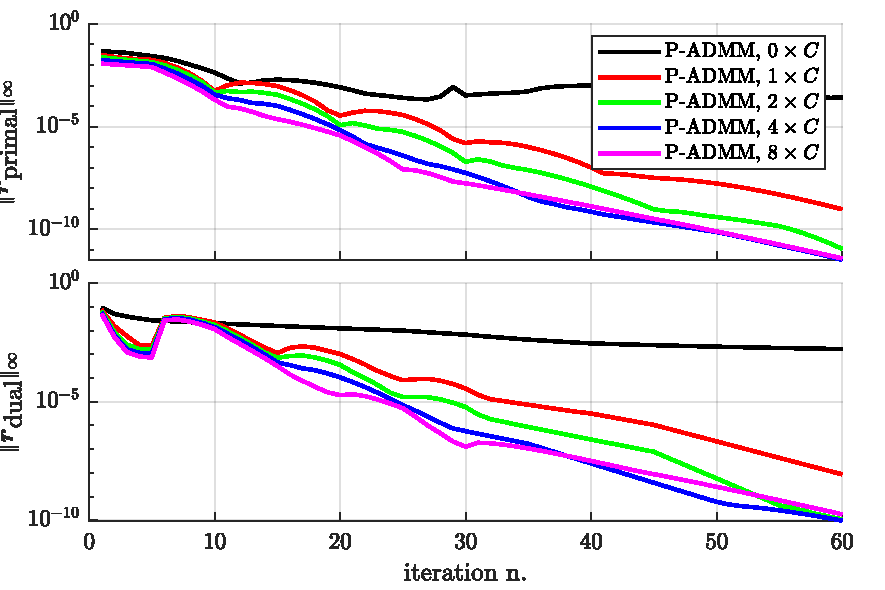
\includegraphics[width=\textwidth]{t8_compliance.pdf}
    \caption{Effect of regularization or compliance in contacts in \textsc{Test 2}.}
  \end{minipage}
\end{figure}


\section{Results and conclusion}

We performed benchmarks involving multi-body systems with contacts between multiple parts, showing that the performance of the ADMM method is capable of handling problems that would converge too slowly using conventional projected fixed point methods or first-order SPG spectral methods \cite{heynIJNME2013}.

Our ADMM method requires few computational primitives: basically a projection of dual variables on conic sets, a backward solve of a linear system, and a forward solve. The latter is a computational bottleneck, but it can be performed only once per run, as the matrix does not change often during the iterations. 
A good estimation of the ADMM step size proved to be fundamental in achieving good convergence: using some heuristics we obtained an efficient auto-tuning algorithm. 
We noted that ADMM can be successfully applied to problems that exhibit temporal coherence because, unlike IPMs, it supports warm-starting. 
Another optimization that allowed superior performance is the adoption of a diagonal preconditioning, with block scaling for the triplets of lagrangian multipliers relative to the conic constraints.

Further research on this topic might address the acceleration of the ADMM method by means of Anderson acceleration.


\bibliographystyle{spmpsci}
\bibliography{../../bibliography/refsMBS,../../bibliography/refsOPT}



\end{document}
